This chapter is adapted from a paper published in \textit{Nucleic Acids Research}, the 2021 Web Server Issue \cite{bhandaribk2021-nar-gkab175}. Associate Professor Paul Gardner, Dr Chun Shen Lim and I conceived the study. Dr Chun Shen Lim and I designed the features of the web server. I developed \href{https://tisigner.com}{https://tisigner.com} and drafted the paper \cite{bhandaribk2021-nar-gkab175}. Drs Gardner and Lim supervised the study.


\section{Abstract}
Experiments that are planned using accurate prediction algorithms will
mitigate failures in recombinant protein production. We have developed
TISIGNER \\(https://tisigner.com) with the aim of addressing technical
challenges to recombinant protein production. We offer three web
services, TIsigner (\underline{T}ranslation \underline{I}nitiation
coding region de\underline{signer}), SoDoPE (\underline{So}luble
\underline{Do}main for \underline{P}rotein \underline{E}xpression) and
Razor, which are specialised in synonymous optimisation of recombinant
protein expression, solubility and signal peptide analysis,
respectively. Importantly, TIsigner, SoDoPE and Razor are linked, which
allows users to switch between the tools when optimising genes of
interest.


\section{Introduction}

Recombinant protein production is a key process for life science
research and the development of biotherapeutics. However, low protein
expression and aggregation are the two major bottlenecks of recombinant
protein production \cite{Berlec2013-mb,Esposito2006-tj,Hou2018-yd,Kramer2012-wk,Mazurenko2020-pr,Rosano2014-oq,Vihinen2020-ar}.
Since mRNA abundance alone is insufficient to explain protein abundance \cite{Bernstein2002-gg,Abreu2009-zf,Lim2018-rq,Nieuwkoop2020-ph,Taniguchi2010-uq},
several features of mRNA sequence have been proposed to affect protein expression. 
These features are mostly related to codon usage, such as
the codon adaptation index and tRNA adaptation index
\cite{Brule2017-mx,Reis2004-dl,Gutman1989-pn,Sabi2014-je,Sharp1987-ed},
or measures of mRNA secondary structure, such as G+C content, minimum
free energy (MFE) of RNA secondary structure, and mRNA:ncRNA interaction
avoidance
\cite{De_Smit1990-xy,Dvir2013-lq,Kudla2009-tl,Plotkin2011-ak,Tuller2015-ts,Umu2016-zq}.
Many of these features are not independent, making it challenging to
distinguish the impacts of individual features
\cite{mauger2019mrna}. This, in turn, hinders
the development of accurate prediction/optimisation tools. Recent systematic 
studies suggest that MFE is the most important feature in
protein expression \cite{Cambray2018-kn,mauger2019mrna}. However, more 
recent work shows that the mRNA accessibility of translation initiation sites 
outperforms MFE in predicting relative protein levels from mRNA sequences
\cite{Bhandari2021-wd,Terai2020-co}. Accessibility
is computed by considering all possible structures for a region,
weighted by free energy, not just the single structure with the MFE \cite{Bernhart2006-ma}.

In addition to high protein expression level, high solubility is
preferable for the purification and long-term storage of recombinant
proteins. However, almost half of the successfully expressed proteins
are insoluble
(\href{http://targetdb.rcsb.org/metrics}{http://targetdb.rcsb.org\\/metrics}),
which makes the recombinant protein production process challenging. A
number of methods have been suggested to improve protein solubility, for
example, truncation, mutagenesis, and the use of solubility-enhancing
tags \cite{Chan2010-mo,Costa2014-oe,Esposito2006-tj,Waldo2003-ui}. 
Nevertheless, accurate solubility prediction could save
resources and aid in designing soluble proteins before the experiments.
With these in mind, we have recently formulated the Solubility-Weighted
Index (SWI), which outperforms recent solubility prediction tools based
on machine-learning algorithms
\cite{Bhandari2020-pz}.

Besides, many recombinant proteins of interest are secretory. The
intracellular accumulation of heterologous secretory proteins may be
toxic to the host cells. Therefore, the translocation efficiency of
these proteins plays an important role in the yield quantity and
quality. Secretory proteins usually have a short peptide at the
N-terminus called Signal Peptide (SP) which is responsible for the 
translocation of secretory proteins via the Sec, Signal Recognition Particle
(SRP) or Twin arginine transport (Tat) pathways
\cite{Luirink1994-br,Palmer2012-cw,Rusch2007-it,Von_Heijne1990-sb}.
Detection of SPs or fusion of a suitable SP at the N-terminus is useful
for optimising protein production
\cite{Freudl2018-lr,Karyolaimos2020-gg,Rosano2019-sj,Zamani2015-xj}. In
addition, different pathways have different advantages, for example, the
SRP dependent pathway can be used for rapidly folding proteins
\cite{Owji2018-hg}. However, the Sec dependent
pathway, which is common across all forms of life, has been widely used
for recombinant protein expression because of higher protein production
capacity and quality
\cite{Ma2018-iz,Owji2018-hg}. In addition, the
presence of SPs should almost always be checked when planning the
expression experiments for uncharacterised proteins.

% **************************************************************
% Keep this command to avoid text of first page running into the
% first page footnotes
% \enlargethispage{-65.1pt}
% **************************************************************

Existing web tools predict or optimise either protein expression or
solubility alone
\cite{Agostini2014-te,Chin2014-wu,Grote2005-vr,Puigbo2007-oj,Hebditch2017-bg,Hon2020-gk,Smialowski2012-yg,Sormanni2015-yr,Zayni2018-wc}.
There also exists several web tools for predicting SPs
\cite{Almagro_Armenteros2019-vr,Bagos2009-wh,Hiller2004-gc,Kall2004-te,Savojardo2017-ux}.
Only a very few tools can detect toxic proteins, for example, SpiderP, ClanTox,
and ToxinPred \cite{Gupta2013-fw,Naamati2009-uf,Wong2013-qh}. 
These tools are either limited to predicting the
venoms of certain organisms, such as spiders, or they are not designed
to predict the signal peptides of toxins, rather to predict the toxicity
of mature peptides.
Moreover, these tools are offered through different independent
services. We reasoned these functionalities should be integrated in
order to assist not only in choosing appropriate expression systems, but
also in optimising the expression and solubility levels of recombinant
proteins. Here we present TISIGNER.com that integrates the optimisation
tools TIsigner (\underline{T}ranslation \underline{I}nitiation coding
region de\underline{signer}), SoDoPE (\underline{So}luble
\underline{Do}main for \underline{P}rotein \underline{E}xpression) for
protein expression and solubility, respectively, and Razor for detecting
SPs \cite{Bhandari2021-wd,Bhandari2020-pz,Bhandari2020-oj}. Our web application provides easy, fast and interactive ways to
assist users in planning and designing their experiments (Figure \ref{fig:nar_webserver_fig_1}).

\begin{figure*}[!hbtp]
\begin{center}
\makebox[\textwidth][c]{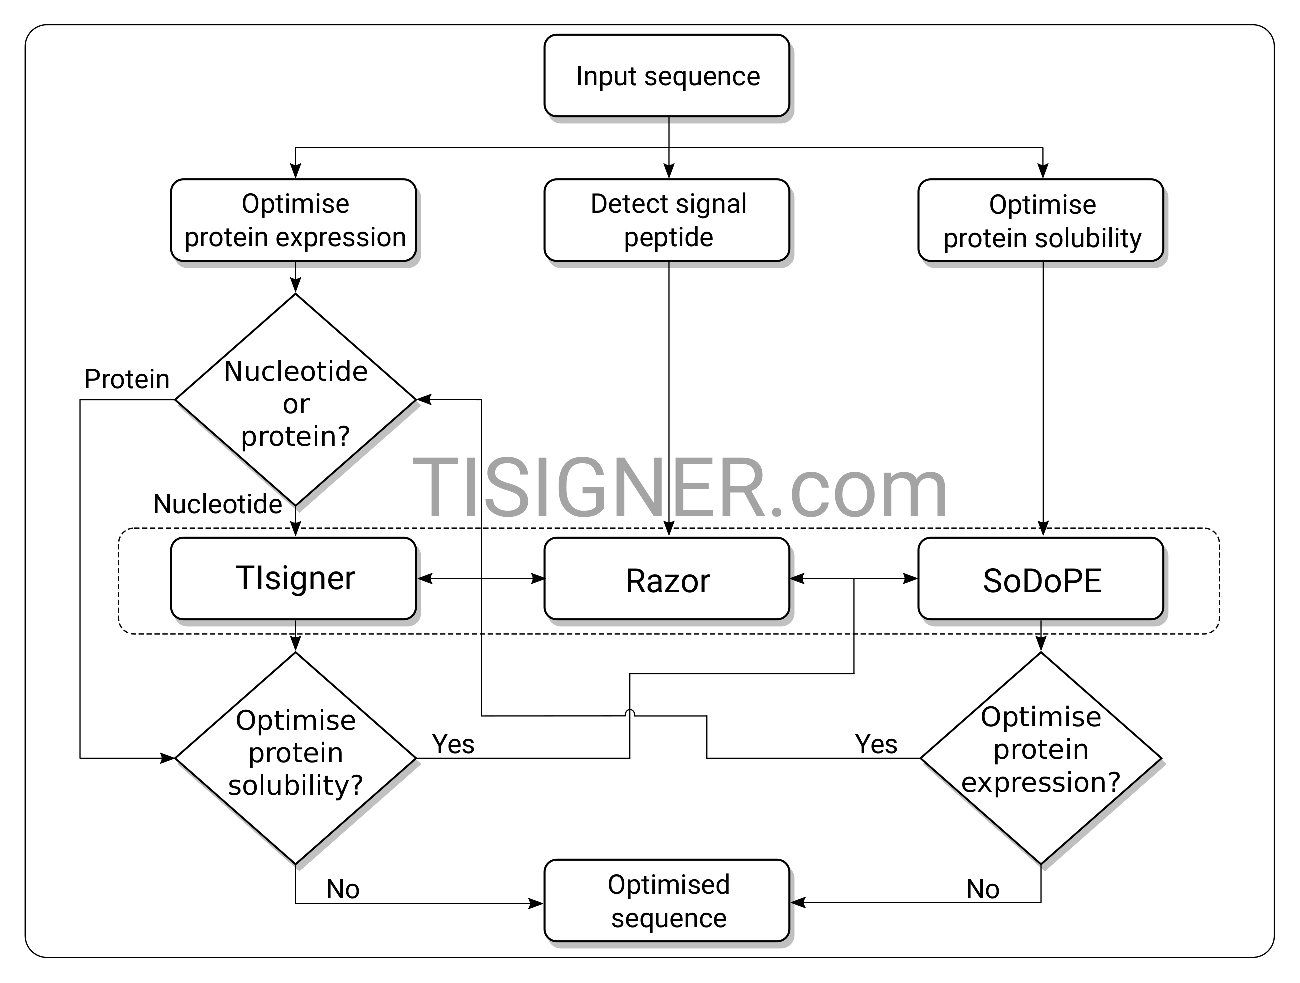
\includegraphics[width=1\textwidth]{chapters/TIsigner_Web/Fig/fig1.eps}}%
\end{center}
\caption[Flow chart for optimising recombinant protein production
using the TISIGNER web application.]{Flow chart for optimising recombinant protein production
using the TISIGNER web application. TIsigner, SoDoPE and Razor are
linked so that protein expression and solubility can be seamlessly
optimised. TIsigner accepts a nucleotide sequence as input, whereas
SoDoPE and Razor accept either a nucleotide or protein sequence. SoDoPE,
\underline{So}luble \underline{Do}main for \underline{P}rotein
\underline{E}xpression; TIsigner, \underline{T}ranslation
\underline{I}nitiation coding region de\underline{signer}.}
\label{fig:nar_webserver_fig_1}
\end{figure*}


\section{Web services}

\subsection{TIsigner}

TIsigner offers tunable protein expression by optimising the mRNA
accessibility of translation initiation sites
\cite{Bhandari2021-wd}. The regions used to
calculate accessibility (opening energy) are specific to the expression
hosts, which is calculated using RNAplfold
\cite{Bernhart2006-ma,Bernhart2011-cc,Lorenz2011-rg}. For
\emph{Escherichia coli}, \emph{Saccharomyces cerevisiae}, and \emph{Mus
musculus} expression hosts, the optimal regions relative to the start
codon for optimisation are $-24:24$, $-7:89$, $-8:11$, respectively. For other
expression hosts, we provide an option `Other', which optimises the
accessibility of the region $−24:89$. Since \emph{E. coli} is the most
popular expression host, the default settings aim to optimise protein
expression in \emph{E. coli} with the T7 lac promoter system (see
below). In this case, only the protein coding sequence is required for
input (Figure \ref{fig:nar_webserver_fig_1}). Otherwise, the 5$^{\prime}$UTR (5$^{\prime}$ 
untranslated region) sequence is also required.



\begin{figure}[!hbtp]
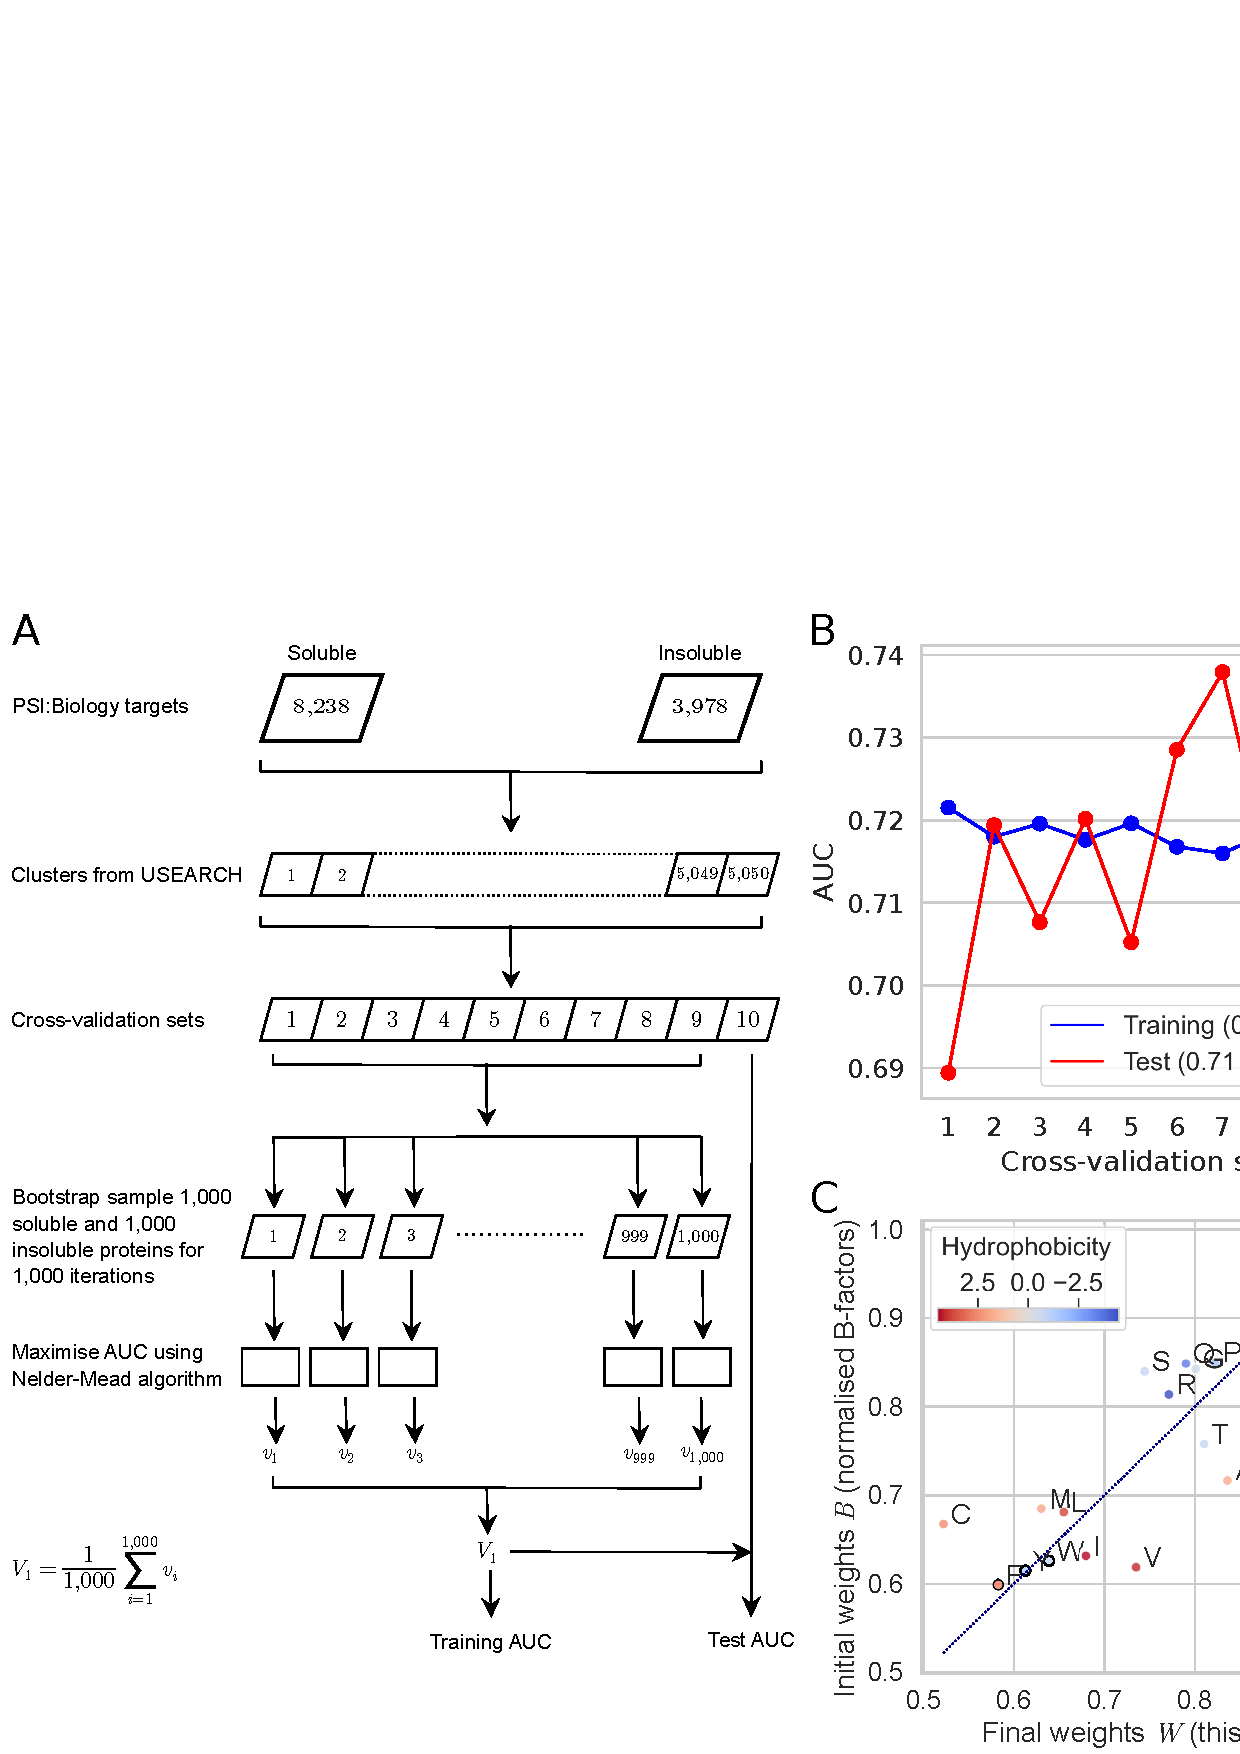
\includegraphics[width=1\textwidth]{chapters/TIsigner_Web/Fig/fig2.pdf}
\caption[The results of TIsigner shows a protein
expression optimised nucleotide sequence.]{The results of TIsigner shows a protein
expression optimised nucleotide sequence. The highlighted nucleotides
show changes made to the input sequence. The opening energy of the input
sequence before and after optimisation is annotated over the
distributions of the opening energy for 8,780 `success' and 2,650 `failure'
experiments from PSI:Biology. Further optimised sequences, if found, are
also displayed. The results can be downloaded in either CSV or PDF
format using the download icon on the bottom right. Each resulting
sequence can be analysed for solubility or signal peptide.}
\label{fig:nar_webserver_fig_2}
\end{figure}

The settings for TIsigner are grouped by complexity (i.e., general,
extra, and advanced). The general settings include the options to modify
the expression host, promoter and target expression score. The target
expression score ranges from $0$ to $100$ (i.e., from the minimum to 
maximum predicted level), which is derived from a logistic regression of 
the opening energy distribution of $11,430$ expression experiments in 
\emph{E. coli} from the `Protein Structure Initiative:Biology' (PSI:Biology) 
\cite{Chen2004-cp,Seiler2014-on}. Hence, this scoring system is only 
applicable to the \emph{E. coli} T7 lac promoter system. Since, there is a non-linear relationship between opening energy and expression score, an interactive plot is also displayed along with the slider to set the target expression score. For other expression 
hosts and promoters, the target expression level can be either maximised or 
minimised (i.e., binary). The extra settings have the options to optimise 
sequence within the translation initiation region or the full-length sequence. 
The AarI, BsaI, BsmBI restriction modification sites are filtered by default, 
whereas other sites can be manually supplied (e.g., a Shine-Dalgarno motif or terminator U-tract). 
The advanced settings allows users to tweak the random seed and sampling 
options (i.e., quick or deep, which uses different numbers of iterations and 
parallel processes). Here users can also customise the region for optimisation 
or disable the terminator checks.

Once the input sequence passes a sanity check, the optimisation task is
rapid ($O(1)$ time using RNAplfold v2.4.11 (using parameters -W
$210$ -u $210$)) with our simulated annealing algorithm. A list of optimised
sequences are returned after checking for terminators using cmsearch
(Infernal v1.1.2)
\cite{Nawrocki2013-te} with RMfam models
\cite{Gardner2015-ui,Kalvari2021-ck}. If
terminators are found, an option to use the full-length sequence for
optimisation will be prompted to users. In a default case (\emph{E.
coli} T7 lac promoter system), the optimised sequence closest to the
chosen expression level is selected as the first solution (Figure \ref{fig:nar_webserver_fig_2}). For other
expression hosts and/or promoters, the optimised sequence with the
minimum changes in nucleotides is selected as the first solution. The
altered nucleotides are highlighted (Figure \ref{fig:nar_webserver_fig_2}). The accessibility of translation
initiation sites for both the input and optimised sequences is shown as
opening energy (kcal/mol). The results can be exported as a PDF or CSV
file. When the default settings are used, the opening energy for each
sequence is indicated on the distributions of the opening energy of
$8,780$ `success' and $2,650$ `failure' groups of the PSI:Biology target
genes. Furthermore, options for solubility and SP analyses using SoDoPE and 
Razor, respectively, are available for each sequence on
the same results page (Figure \ref{fig:nar_webserver_fig_2}).


\subsection{SoDoPE}

SoDoPE is our interactive solubility analysis and optimisation tool
based on the Solubility-Weighted Index (SWI)
\cite{Bhandari2020-pz}. SoDoPE accepts either
a nucleotide or protein sequence (Figure \ref{fig:nar_webserver_fig_1}). Upon submission, a query is
sent to the HMMER web service for domain annotation
\cite{Potter2018-ox}. Successful annotations
are displayed as interactive graphics, in which the annotated domains
are represented as discorectangles, above a grey band that represents
the input protein sequence (Figure \ref{fig:nar_webserver_fig_3}). Information about a protein domain is shown
upon a mouse hover. The domains can be selected for solubility
analysis. For a complete domain annotation report, a link to the HMMER
results page is also provided.

\begin{figure}[!hbtp]
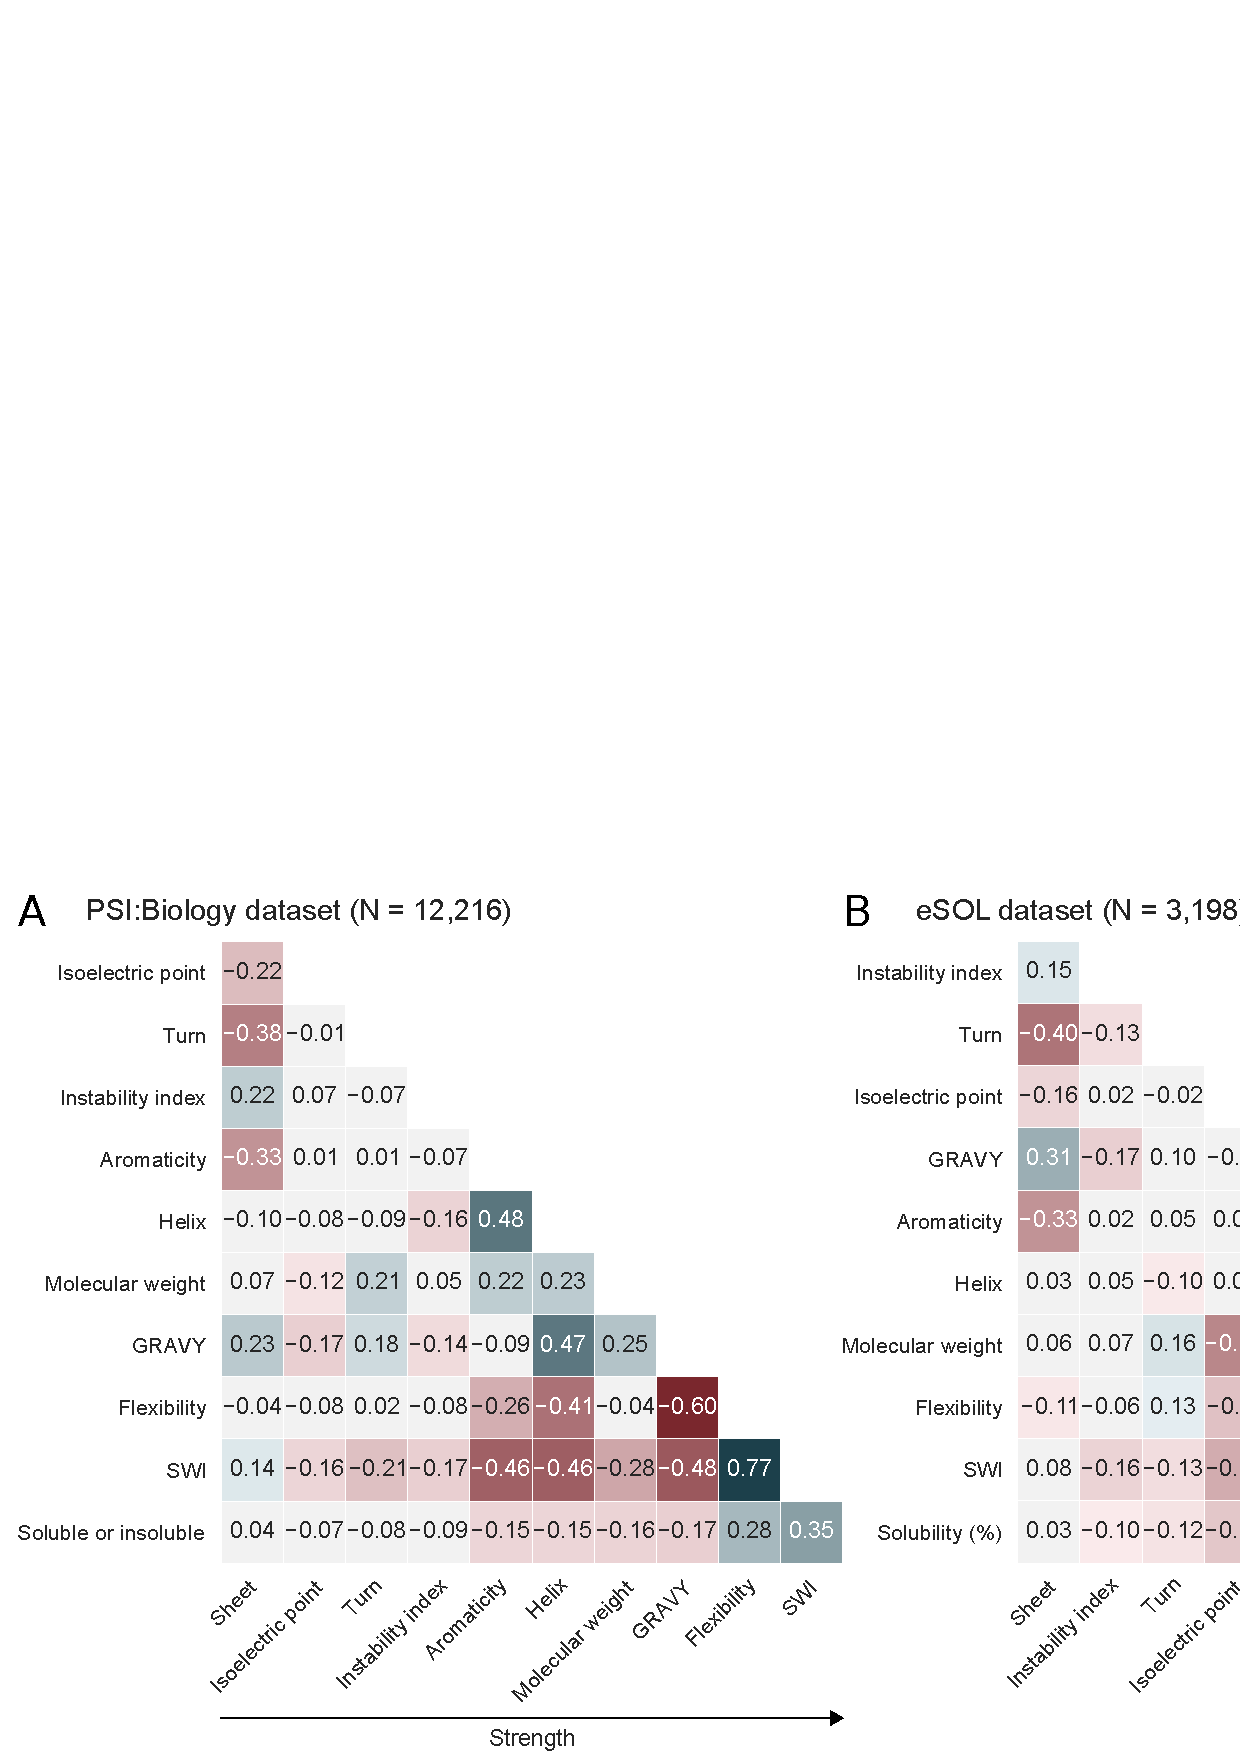
\includegraphics[width=1\textwidth]{chapters/TIsigner_Web/Fig/fig3.pdf}
\caption[Exploring and optimising protein solubility using SoDoPE interactive
graphics.]{Exploring and optimising protein solubility using SoDoPE interactive
graphics. Upon clicking a protein domain or selecting a region of
interest, its solubility is optimised in real-time, and a list of
regions with extended boundaries and higher probabilities of solubility
is returned as green buttons (clickable). The probabilities of
solubility of the selected region with and without fusion tags can be
visualised in a barplot. The flexibility and hydrophobicity profile
plots for the selected region can also be selectively viewed. The
sequence can also be checked for the presence of a signal peptide or
optimised for protein expression.}
\label{fig:nar_webserver_fig_3}
\end{figure}

In addition, a two-way slider is available for navigation through any
region of interest (Figure \ref{fig:nar_webserver_fig_3}). The probability of solubility, flexibility and GRAVY
(GRand AVerage of hydropathicitY) is shown in real-time according to the
user-selected region. The selected region is optimised for higher
solubility using simulated annealing. Only the regions with extended
boundaries and also higher probability of solubility is returned. SP
analysis can also be done using Razor (see below).

A profile plot of flexibility and/or hydrophilicity corresponding to the
user selected region is generated (Figure \ref{fig:nar_webserver_fig_3}). This allows an estimation of
rigid/flexible regions and possible helices, that may be helpful for
mutagenesis experiments. The sequence of the selected region is shown,
with the option of sequence conversion between nucleotide and amino acid
sequence format. In particular, the nucleotide sequence can be
redirected to TIsigner for optimising protein expression (Figure \ref{fig:nar_webserver_fig_1} and \ref{fig:nar_webserver_fig_3}, through the `view DNA \textbar\ optimise expression' button).

The contributions of several solubility-enhancing tags to user selected
regions can be compared and shown in a bar plot, including thioredoxin
(TRX), maltose binding protein (MBP), small ubiquitin-related modifier
(SUMO) and glutathione S-transferase (GST) tags (Figure \ref{fig:nar_webserver_fig_3}). Users can also input a
fusion sequence of interest either in a nucleotide or protein sequence
format.

% **************************************************************
% Keep this command to avoid text of first page running into the
% first page footnotes
% \enlargethispage{-65.1pt}
% **************************************************************

\subsection{Razor}

Razor is our SP prediction tool which is based upon random forest models
of protein features from the eukaryotic SP sequences of the SignalP 5.0
dataset and the animal toxin annotation project
\cite{Almagro_Armenteros2019-vr,Bhandari2020-oj,Jungo2012-ja}. Razor accepts
either a protein or a nucleotide sequence (Figure \ref{fig:nar_webserver_fig_1}). After validation, the
N-terminal region is checked for the presence of a SP using five random
forest models. This gives five SP scores (S-scores) for a given
sequence. For detecting the cleavage site, we use a sliding window of $30$
residues and our optimised weight matrix for residues around the
cleavage site. The scored subsequences are scored by additional five
random forest models to give the cleavage site scores (C-scores) along
the sequence, which is displayed as a step plot (Figure \ref{fig:nar_webserver_fig_4}). The Y-score, which is
the geometric mean of S-scores and the max of C-scores, is used to infer
whether the given sequence has a SP or not. The median of these five
Y-scores is displayed as the final score. The cleavage site from the
model with the median of max of C-scores is used to annotate the
predicted region.

\begin{figure}[!hbtp]
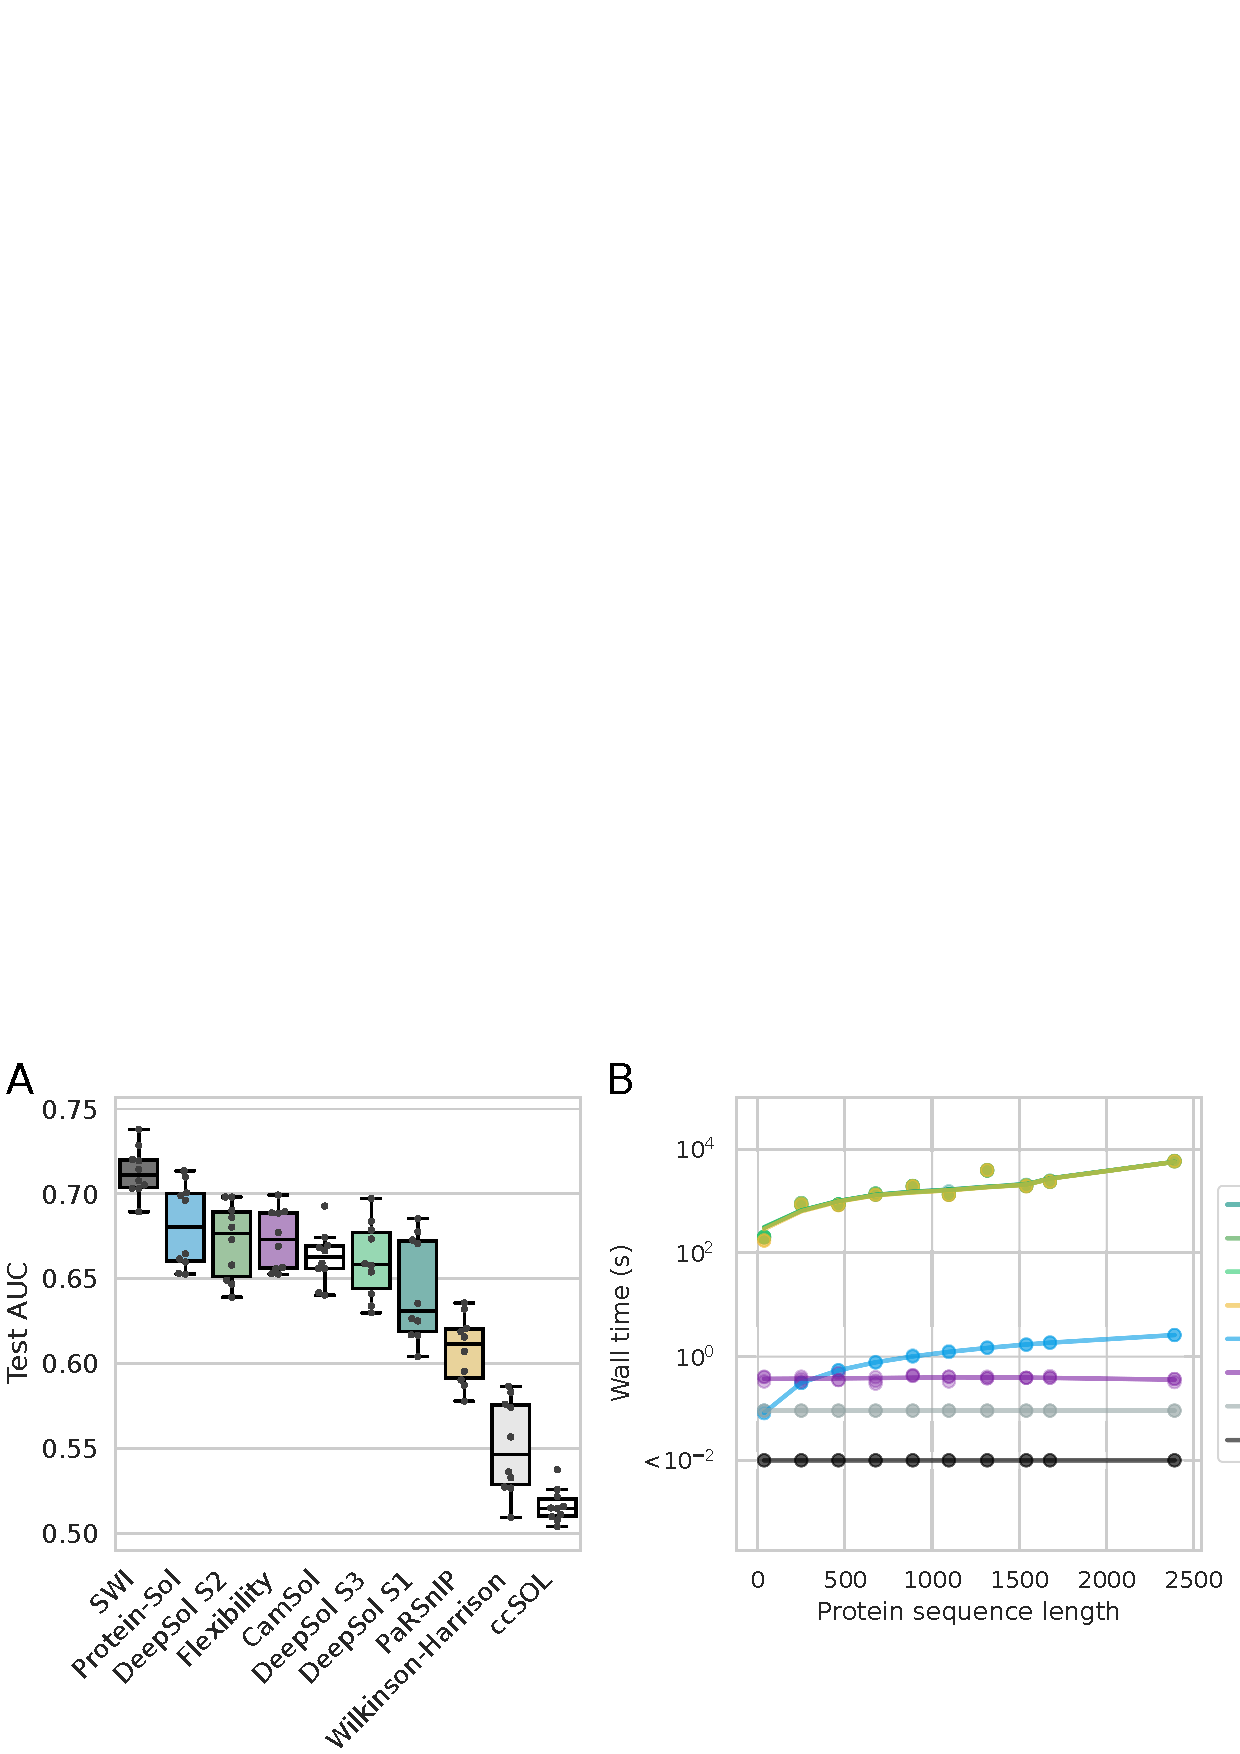
\includegraphics[width=1\textwidth]{chapters/TIsigner_Web/Fig/fig4.pdf}
\caption[Detection of signal
peptides using Razor.]{Detection of signal
peptides using Razor. The dotted annotation in the step plot for the
cleavage site scores (C-scores) shows the most likely position for
proteolytic cleavage. The sequence can also be checked and optimised for protein
solubility and expression.}
\label{fig:nar_webserver_fig_4}
\end{figure}


If any of the models detect a SP in the input sequence, we further check
whether the SP belongs to toxins, using five random forests trained on
toxin-specific SPs. The final toxin score is the median of scores from
those random forest models. Furthermore, since we noticed a lack of
tools specialising in predicting SPs from fungi, any detected signal
peptide is checked for such origin. Similarly, we use five random
forests for detecting fungal SPs, with the final fungal score being the
median score of these models. This random forest is built using residue composition of the signal sequence. Since we have five random forest models in
each step (SP, toxin- and fungal-specific SP detection steps), stars are displayed as an
indication of the number of models agreeing on the sequence falling on
either category (Figure \ref{fig:nar_webserver_fig_4}).

Razor is linked with SoDoPE for checking and optimising protein
solubility (Figure \ref{fig:nar_webserver_fig_4}). If a nucleotide sequence was submitted, this sequence can
also be optimised for protein expression using TIsigner (Figure \ref{fig:nar_webserver_fig_1}).


\section{Discussion}
Low protein expression and solubility are the major hindrances to a successful recombinant protein production. Based on our comprehensive studies on these two problems, we have developed novel tools to optimise protein expression (TIsigner) and solubility (SoDoPE), and assessed their predictive performance using independent datasets (Table \ref{tab:Summary_of_TIsigner_and_SoDoPE}). Our tools offer some unique features in an interactive way. TIsigner allows tuning of protein expression from low to high levels, whereas SoDoPE allows easy navigation of protein sequence/domains with real-time solubility prediction. Based on our assessment of similar tools, none of the publicly available tools provides these features.

Our third tool, Razor, is designed to check the presence of SPs. Compared to other related tools, Razor also predicts toxin- and fungal-specific SPs (Table \ref{tab:Summary_of_Razor}). These would be helpful for users in choosing the expression and purification systems that prevent the harmful intracellular accumulation of recombinant secretory proteins/toxins. 

Our tools are interactive, fast, and accurate. Importantly, our tools are highly integrated, allowing a seamless transition between the optimisation tools. To make such transition intuitive, our web services limits one input sequence at a time and we aim to remove this input sequence limitation in the future. For optimising a large number of sequence, we provide the command-line version of each of our tools (see below).


\section{General information}

Demo input and results are available for new users to get started. A
list of frequently asked questions is also available for each tool. The
frontend is written in React and uses responsive web design principles.
The backend is written in Flask and Python v3.6. The website is hosted on
a virtual machine (Red Hat Enterprise Linux 8) running on Intel Xeon (8
${\times}$ 2.60 GHz) with 4GiB RAM, by the Information Technology Services at the
University of Otago.


\section{Data availability}

The web server is available at \href{https://tisigner.com}{https://tisigner.com}. This website is free
and open to all users and there is no login required. All our tools, and the website 
are open-sourced (\href{https://github.com/Gardner-BinfLab/TISIGNER-ReactJS}{https://github.com/Gardner-BinfLab/TISIGNER-ReactJS};\\ \href{https://github.com/Gardner-BinfLab/TIsigner/tree/master/TIsigner\_cmd}{https://github.com/Gardner-BinfLab/TIsigner/tree/master/TIsigner\_cmd};\\ \href{https://github\\.com/Gardner-BinfLab/SoDoPE\_paper\_2020/tree/master/SWI}{https://github.com/Gardner-BinfLab/SoDoPE\_paper\_2020/tree/master/SWI};\\ \href{https://github.com/Gardner-BinfLab/Razor}{https://github.com/Gardner-BinfLab/Razor}) and privacy friendly (no user data stored).


% \section{Acknowledgements}

% This work was supported in part by the Ministry of Business, Innovation
% and Employment {[}MBIE Smart Idea grant: UOOX1709 and MBIE Data Science
% Programmes grant: UOAX1932{]}, and the Royal Society of New Zealand Te
% Apārangi {[}Marsden grant: 19-UOO-040{]}.